\documentclass{beamer} % [handout] para imprimir eliminando transiciones

%\usefonttheme[onlymath]{serif}
%\usepackage{fontspec}
%\defaultfontfeatures{Mapping=tex-text}
%\setsansfont[Ligatures={Common}]{Futura}
%\setmonofont[Scale=0.8]{Monaco} 

\usepackage{beamerthemesplit}
\usepackage[utf8]{inputenc}
\usepackage[spanish]{babel}
\mode<presentation>
\usetheme{default}
\usecolortheme{dolphin}
\usepackage{alltt}                                    % \begin{alltt}
\usepackage{amssymb}                                  % mathematical symbols
\usepackage{comment}
\usepackage{tabto}                                    % \tabto
\usepackage{tikz}
\usetikzlibrary{automata}
\usetikzlibrary{positioning}
\usetikzlibrary{calc}

\usepackage{verbatim}                                 % comentarios

\title{Lenguajes de Programación}                     %[titulo corto]
\author{Fabián Riquelme Csori}                        %[nombre corto]
\date{2017}                                           %[fecha corta]
\institute{Universidad de Valparaíso}                 %[instituto corto]

\newcommand{\HRule}{\rule{\linewidth}{0.2mm}\\[1ex]}
\newcommand{\blue}[1]{\textcolor{blue}{#1}}
\newcommand{\red}[1]{\textcolor{red}{#1}}
\newcommand{\redb}[1]{{\color{red!70!black}{#1}}}
\newcommand{\green}[1]{{\color{green!70!black}{#1}}}
\newcommand{\gray}[1]{{\color{gray!50!white}{#1}}}
\newcommand{\yell}[1]{{\color{yellow!70!black}{#1}}}
\newcommand{\lQ}{\mbox{``}}
\newcommand{\rQ}{\mbox{''}}
% \alert{texto destacado en rojo}
% \color{green} Color en verde
% \structure{texto en lila}


\begin{document}

%\begin{frame}%[plain]
%  \titlepage
%\end{frame}
%
% [opciones]:
% plain: oculta barra de navegacion, deja + espacio para contenido
% fragile: usar comandos como verbatim
% b,c,t: alineacion vertical
% label=nombre_etiqueta
% allowframebreaks: divide contenido en varios frames si es demasiado largo
% shrink: para escribir mucho texto en una transparencia, reduciendo tamano de fuente

%%%%%%%%%% PORTADA %%%%%%%%%%
\begin{frame}[plain]
  \begin{figure}[h]
    \begin{minipage}{0.3\textwidth}
    
\includegraphics[width=.9\textwidth]{./image/logo-UV.png}
    \end{minipage}
    \begin{minipage}{0.65\textwidth}
     $~$\\[3.6ex]
     \footnotesize{Escuela de Ingeniería Civil Informática}\\
     \footnotesize{Facultad de Ingeniería}
    \end{minipage}
  \end{figure}
  \begin{center}
    \vspace{1ex}
    \HRule
    \Large{Lenguajes de Programación}\\{\small Capítulo IV: Programación funcional}\\[-1ex]
    \HRule\vspace{1ex}
    \large{Fabián Riquelme Csori}\\[.5ex]\footnotesize{fabian.riquelme@uv.cl}\\[6ex] {\tiny 2017-II}\\[6ex]
  \end{center}
\end{frame}

%%%%%%%%%% INDEX %%%%%%%%%%
\begin{frame}
 \frametitle{Index}
 \scriptsize 			% reducir tamano de letra
 \tableofcontents		%[pausesections]
\end{frame}

%%%%%%%%%%% ACTUAL INDEX %%%%%%%%%%
%\AtBeginSection[] %generar indice automaticamente
%{
%\begin{frame}<beamer>%[plain]
% \frametitle{Index}
% \framesubtitle{subtitulo}
% \scriptsize
% \tableofcontents[currentsection, currentsubsection]
%\end{frame}
%}

%==============================
\section{Fundamentos}

%------------------------------
\subsection{Paradigma funcional}

\begin{frame}{El paradigma funcional}
  \begin{itemize}
    \item La \blue{programación funcional} es un paradigma de \blue{progamación declarativa}.
    \begin{itemize}
        \item Al contrario de la \blue{programación imperativa}, que especifica el ``cómo'', la declarativa se centra en el ``qué''.
    \end{itemize}
    \item Basada en las funciones matemáticas y el \blue{Lambda calculus}:
    \begin{itemize}
        \item Sistema formal para definir una \blue{función computable}.
        \item Creado por A. Church y S. Kleene en los 1930s.
        \item Con $\lambda$-calculus, Church resolvió en 1936 el {\em Entscheidungsproblem}, en paralelo a A. Turing.
    \end{itemize}
  \end{itemize}
\end{frame}

\begin{frame}{Ejemplo: Programación procedural (imperativa)}
  \texttt{function OddWordsVerifier(words) \{}\\
  $~~~~$\texttt{var result = true;}\\
  $~~~~$\texttt{for (var i = 0; i < length(words); ++i) \{}\\
  $~~~~~~~~$\texttt{var len = length(words[i]);}\\
  $~~~~~~~~$\texttt{if (!odd(len)) \{}\\
  $~~~~~~~~~~~~$\texttt{result = false;}\\
  $~~~~~~~~~~~~$\texttt{break;}\\
  $~~~~~~~~$\texttt{\}}\\
  $~~~~$\texttt{\}}\\
  $~~~~$\texttt{return result;}\\
  \texttt{\}}
  \pause
  \begin{itemize}
    \item Alta variabilidad en el valor de variables.
    \item Asignaciones de variables pueden cambiar a posteriori.
    \item Explicita ``cómo'': operaciones necesarias para generar output.
  \end{itemize}
\end{frame}

\begin{frame}{Ejemplo: Programación funcional (declarativa)}
  \texttt{function OddWordsVerifier(words) \{}\\
  $~~$\texttt{return apply(and, map(compose(odd, length), words));}\\
  \texttt{\}}\\
  \begin{itemize}
    \item<2-> De dentro hacia afuera, la función:
    \begin{itemize}
        \item<2-> \texttt{compose}: determina si el largo de un string es impar.
        \item<2-> \texttt{map}: retorna lista de booleanos con respuestas para cada string. Esta función sustituye el iterador.
        \item<2-> \texttt{apply}: aplica un ``and'' a lista resultante para generar output.
    \end{itemize}
    \item<3-> Explicita el ``qué'': combinación de funciones para pasar del input al output.
    \item<4-> Los resultados parciales dependen exclusivamente de parámetros de cada función (no hay efectos secundarios).
  \end{itemize}
\end{frame}

%------------------------------
\subsection{Ventajas y desventajas}

\begin{frame}{Ventajas y desventajas}

  \blue{Ventajas}
  \begin{itemize}
    \item<2-> Códigos en general más compactos.
    \item<3-> Facilita el análisis de rendimiento del algoritmo y precedir su comportamiento.
    \item<4-> Útil para implementar simulaciones de estados, problemas de optimización y aplicaciones en contextos académicos.
  \end{itemize}
  \uncover<5->{\blue{Desventajas}}
  \begin{itemize}
      \item<6-> En general son menos eficientes que los lenguajes imperativos (C, C++, PHP, Python, etc.)
      \item<7-> En general mucho menos usado en la industria.
  \end{itemize}
\end{frame}

\begin{frame}{}
  \begin{center}
    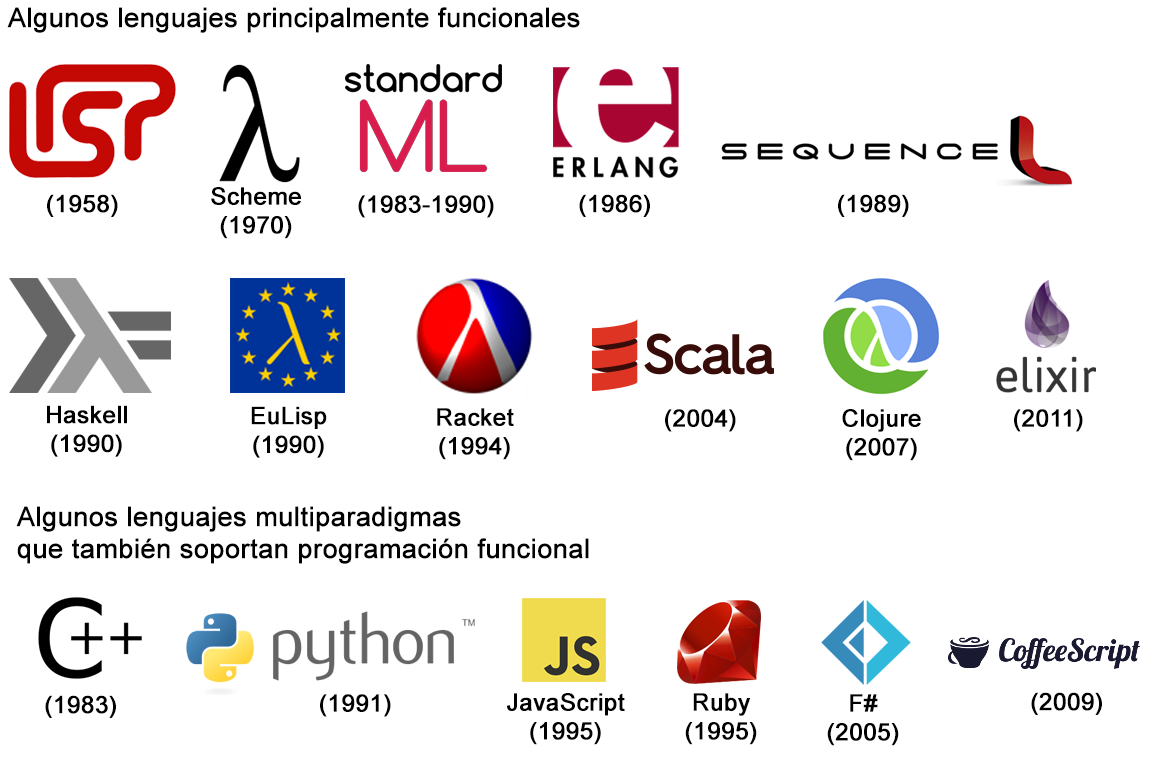
\includegraphics[width=\textwidth]{./image/cap4/lengfuncionales.png}
  \end{center}
\end{frame}

%==============================
\section{Características}

%------------------------------
\subsection{Funciones de primera clase}

\begin{frame}{Funciones de orden superior}
    Una \blue{función de orden superior} ({\em higher-order function}) es una función capaz de:
    \begin{itemize}
        \item Recibir funciones como argumentos, o bien
        \item Retornar una función como resultado.
    \end{itemize}
    \medskip\pause
    
    Ej: \pause $\frac{\blue{d}f(x)}{\blue{dx}}=f'(x)$
    \medskip\pause
    
    Ej:
    \footnotesize{
    $~$ \texttt{\$twice = \green{function}(\$f, \$v) \{}\\
    $~~~~~~~~~~~$ \texttt{\green{return} \$f(\$f(\$v));}\\
    $~~~~~~~~$\texttt{\};}\\
    $~~~~~~~~$\texttt{\$f = \green{function}(\$v) \{}\\
    $~~~~~~~~~~~$ \texttt{\green{return} \$v + 3;}\\
    $~~~~~~~~$\texttt{\};}\\
    $~~~~~~~~$\texttt{\green{echo}(\$twice(\$f, 7)); \gray{// 13}}
    $~~~$ (código escrito en... \pause PHP)
    }\medskip\pause
    
    Ej: Todas las funciones en \blue{$\lambda$-calculus} son de orden superior.
    \medskip\pause
    
    Ej: La función \texttt{map} típica de lenguajes funcionales.
\end{frame}

\begin{frame}{Funciones de primera clase}
    \begin{itemize}
        \item<1-> En lenguajes de programación, un \blue{ciudadano de primera clase} (donde ``ciudadano'' puede ser un objeto, tipo o valor) es una entidad que soporta todas las operaciones generalmente disponibles para otras entidades.
        \item<2-> Estas operaciones incluyen su paso como argumentos, retornos de una función, modificaciones y asignaciones de variables.
        \item<3-> Los lenguajes funcionales soportan \blue{funciones de primera clase}, i.e., las funciones son ciudadanos de primera clase.
    \end{itemize}
    \medskip
    
    \uncover<4->{Ej (SML):\\
      $~~~~$ \texttt{fun echo (s:string):string = s;}\\
      $~~~~$ \texttt{echo("Hello World");}
    }
\end{frame}

%------------------------------
\subsection{Funciones puras}

\begin{frame}{Efectos colaterales}
    \begin{itemize}
        \item<1-> Una función o expresión tiene \blue{efectos colaterales} si además de retornar un valor, modifica algún estado fuera de su alcance.
        \item<2-> Los efectos colaterales son muy frecuentes en los lenguajes de programación imperativos.
        \medskip
        
        \begin{itemize}
            \item Ej (C++):\medskip
            
            $~~~~$ \texttt{\red{int} i, j;}\\
            $~~~~$ \texttt{i = j = 3;} \gray{\texttt{//C++ lee i = (j = 3)}}
        \end{itemize}
    \end{itemize}
\end{frame}

\begin{frame}{Funciones puras}
    \begin{itemize}
        \item<1-> Las funciones de los lenguajes funcionales son \blue{funciones puras}, i.e., no admiten efectos colaterales (ni de memoria ni I/O).
        \begin{itemize}
            \item<2-> Ej: Las funciones \texttt{sin(x)} y \texttt{length(s)} son típicamente funciones puras.
            \item<3-> Ej: Las funciones como \texttt{time()}, \texttt{date()}, \texttt{random()}, o aquellas que usan variables no-locales, son impuras.
            \item<4-> Ojo: \texttt{printf()} es una función impura.
            \medskip
            
            Investigar: ¿Cómo entonces los lenguajes funcionales interactúan con mecanismos de I/O?
        \end{itemize}
    \end{itemize}
\end{frame}

\begin{frame}{Ventajas de las funciones puras}
    
    En programación funcional, el hecho que las funciones sean puras conlleva varias ventajas:
    \begin{itemize}
        \item<1-> Si el resultado de una función no se usa, podemos eliminarla sin miedo de afectar otras funciones.
        \item<2-> Si no hay dependencia entre dos funciones puras, su orden puede invertirse y pueden ejecutarse en paralelo.
        \item<3-> El compilador es libre de evaluar el código mediante cualquier estrategia, reordenando o combinando las evaluaciones a gusto (Ej: \blue{reforestación}).
    \end{itemize}
\end{frame}

\begin{frame}{Ventajas de las funciones puras}
    \begin{itemize}
        \item<1-> \blue{Transparencia referencial}: el resultado de una función es constante con respecto a su lista de argumentos, i.e., podemos reemplazar la función por su valor sin riesgo de cambiar el funcionamiento del programa.
        \begin{itemize}
            \item<2-> Esto permite utilizar muy bien la técnica de optimización llamada \blue{memoización}.
            \item<3-> Ej: la expresión \texttt{x = x * 10} de C y C++ viola la transparencia referencial.
        \end{itemize}
    \end{itemize}
\end{frame}

\begin{frame}{Ventajas de las funciones puras}
    \begin{itemize}
        \item Ej: para el siguiente código:
            \medskip
            
            {\footnotesize
            \texttt{\red{int} globalValue = \gray{0};}\\[1.2ex]
            \texttt{\red{int} \blue{rq}(\red{int} x) \{}\\
            $~~~~$ \texttt{globalValue++;}\\
            $~~~~$ \texttt{\green{return} x + globalValue;}\\
            \texttt{\}}\\[1.2ex]
            \texttt{\red{int} \blue{rt}(\red{int} x) \{}\\
            $~~~~$ \texttt{\green{return} x + \gray{1};}\\
            \texttt{\}}
            }
            \medskip\pause
            
            solo la función \texttt{\blue{rt}} es referencial transparente
            \medskip\pause
            
            \texttt{\blue{rq}(x) - \blue{rq}(x)} $\neq 0$
    \end{itemize}
\end{frame}

%------------------------------
\subsection{Recursión}

\begin{frame}{Recursión}
    \begin{itemize}
        \item En programación funcional, las iteraciones suelen implementarse como \blue{funciones recursivas} que se llaman a sí mismas.
        \item La naturaleza de este paradigma favorece la implementación de algoritmos recursivos.
    \end{itemize}
\end{frame}

\begin{frame}{Recursión}
    
    Ej: código en C para calcular los números de Fibonacci:
    \bigskip
    
    {\scriptsize
    \begin{minipage}{0.48\textwidth}
    \texttt{\green{\#include<stdio.h>}}\\
    \texttt{\redb{int} Fibonacci(\redb{int});}\\[1.2ex]
    \texttt{main() \{}\\
    $~~~~$\texttt{\redb{int} n, i = 0, c;}\\
    $~~~~$\texttt{scanf("\red{\%d}",\&n);}\\
    $~~~~$\texttt{printf("\red{Fibonacci series}\blue{$\backslash$n}");}\\
    $~~~~$\texttt{\yell{for}(c = 1; c <= n; c++) \{}\\
    $~~~~~~~~$\texttt{printf("\red{\%d}\blue{$\backslash$n}", Fibonacci(i));}\\
    $~~~~~~~~$\texttt{i++;}\\
    $~~~~$\texttt{\}}\\
    $~~~~$\texttt{\yell{return} 0;}\\
    \texttt{\}}
    \end{minipage}
    \begin{minipage}{0.48\textwidth}
    \texttt{\redb{int} Fibonacci(\redb{int} n) \{}\\
    $~~~~$\texttt{\yell{if} (n == 0)}\\
    $~~~~~~~~$\texttt{\yell{return} 0;}\\
    $~~~~$\texttt{\yell{else if} (n == 1)}\\
    $~~~~~~~~$\texttt{\yell{return} 1;}\\
    $~~~~$\texttt{\yell{else}}\\
    $~~~~~~~~$\texttt{\yell{return} (Fibonacci(n-1)}\\
    $~~~~~~~~$\texttt{+ Fibonacci(n-2));}\\
    \texttt{\}}
    \end{minipage}}
\end{frame}

\begin{frame}{Recursión}

    Ej: códigos equivalentes en lenguajes funcionales:
    \bigskip

    {\scriptsize
    \begin{minipage}{0.48\textwidth}
    {\bf Elixir}\\
    \texttt{\green{defmodule} \blue{Fibonacci} \green{do}}\\
    $~~$\texttt{\green{def} fib(0), do: 0}\\
    $~~$\texttt{\green{def} fib(1), do: 1}\\
    $~~$\texttt{\green{def} fib(n), do: fib(n-1)+fib(n-2)}\\
    \texttt{\green{end}}\\[1.5ex]
    {\bf Clojure}\\
    \texttt{(\green{defn} fib}\\
    $~~~~$\texttt{[n]}\\
    $~~~~$\texttt{(\green{loop} [a 0 b 1 i n]}\\
    $~~~~~~$\texttt{(\green{if} (\green{zero?} i)}\\
    $~~~~~~~~$\texttt{a}\\
    $~~~~~~~~$\texttt{(\blue{recur} b (+ a b) (\green{dec} i)))))}
    \end{minipage}
    \begin{minipage}{0.50\textwidth}
    {\bf Lisp}\\
    \texttt{(\green{defun} fib (n \green{\&optional} (a 0) (b 1))}\\
    $~~~~$\texttt{(\green{if} (\green{=} n 0)}\\
    $~~~~~~$\texttt{a}\\
    $~~~~~~~~$\texttt{(fib (\green{-} n 1) b (\green{+} a b))))}\\[1.2ex]
    {\bf Lisp}\\
    \texttt{(\green{defun} fib (k)}\\
    $~~~~$\texttt{(\green{if} (\green{zerop} k) || (\green{=} k 1)}\\
    $~~~~~~$\texttt{k}\\
    $~~~~~~$\texttt{(\green{+} (fib (\green{-} k 1)) (fib (\green{-} k 2)))))}\\[1.2ex]
    {\bf SequenceL}\\
    \texttt{\blue{fib}(n) := n when n < 2 \green{else}}\\
    $~~~~$\texttt{fib(n - 1) + fib(n - 2);}
    \end{minipage}}
\end{frame}


%------------------------------

\begin{frame}
 \begin{block}{Bibliografía}
  \begin{itemize}
    \item Pratt, Terrence W. (1998). \textit{Lenguajes de programación: diseño e implementación}, Pearson Education.
    \item Sethi, Ravi (1992). \textit{Lenguajes de programación: conceptos y constructores}, Addison-Wesley Iberoamericana.
    \item Scott, Michael (2009). \textit{Programming Language Pragmatics}, Morgan Kaufman, 3ra ed.
  \end{itemize}
 \end{block}
 \begin{block}{Recursos}
  \begin{itemize}
    \item Wikipedia y Wikimedia Commons.
    \item Imágenes con licencia libre.
  \end{itemize}
 \end{block}
\end{frame}

\end{document}
